% % % % % % % % % % % % % % % % % % % % % % % % % % % % % % % % % % % % % % % % 
% Formelsammlung von LaTeX4EI									
%
% @encode: 	UTF-8, tabwidth = 4, newline = LF
% @author:	Emanuel Regnath
% @date:		
%
% % % % % % % % % % % % % % % % % % % % % % % % % % % % % % % % % % % % % % % % 

%---------------------------------------%
%			P R E A M B L E				%
%~~~~~~~~~~~~~~~~~~~~~~~~~~~~~~~~~~~~~~~%

% Document Class ===============================================================
\documentclass[fs, footer]{latex4ei}

\usepackage{latex4ei_unicode}
\usepackage{multirow}

\usepackage[mathletters]{ucs}




% Dokumentbeginn
% ======================================================================
\begin{document}


% Aufteilung in Spalten
\begin{multicols}{4}
% -----------------------------------------------
% | 			Musikalische Akustik				|
% ~~~~~~~~~~~~~~~~~~~~~~~~~~~~~~~~~~~~~~~~~~~~~~~
%===============================================================================================================================

% Prüfung: Mündlich, 30 min
% 3 aus den 5 Themen

% Exkursion: 26.06.14
% 15:00 an der Musikhochschule München (südlicher Eingang)
% Prof. Christian Böhm



% Interessant: Chladni Patterns,




% Prüfung:
% 11. 14. 15. 16. Juli
% Wichtig für Prüfung: Skript, Exkursion


% Tonhöhenunterschiede lassen sich mit Obertönen besser erkennen, da unterschiede größer werden.



\fstitle{Akustik}
% =====================================================================




% ##########################################################################
\section{Musiktheorie}
% ##########################################################################

\begin{center}
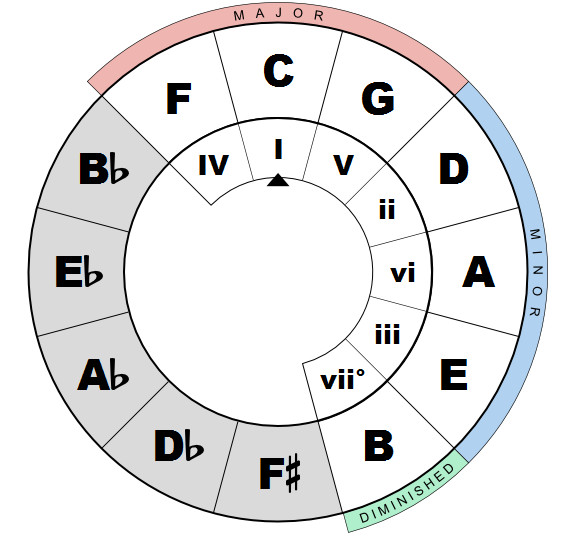
\includegraphics[width=0.7\columnwidth]{./img/circle-of-fifths.jpg}
\end{center}

\sectionbox{
\subsection{Stimmungen}
Funk-A: 443 Hz\\
Mittelalter: reine Stimmung\\
Bach: Wohltemperierte Stimmung (=Werckmeister Stimmung)\\
Heute: gleichschwebende Stimmung: 1HT $=\sqrt[12]{2} = 1.06$\\
12 Quinten sind nicht genau 7 Oktaven: $1.5^{12} \ne 2^7$
}



\sectionbox{
\subsection{Gehör}
Absolutes Gehör: $\SI{440}{\hertz}\pm 6\%$ erkennen.\\
Relatives Gehör: Tonintervall (Tertz, Quint) erkennen.
}


% ##########################################################################
\section{Akustik von Musikinstrumenten}
% ##########################################################################

\sectionbox{
\subsection{Streicher (klassisches Orchester) ($\lambda/2$)}
Violinen: Senkrechter Winkel vom Hals weg, Quintenabstand\\
Gamben: Hängende Schultern bzw. schräger Winekl vom Hals weg, Quartabstand\\
\\
Violine/Geige: $g_3$, $d_4$, $a_4$, $e_5$\\
Viola/Bratsche: $c_3$, $g_3$, $d_4$, $a_4$\\
Violoncello/Cello: $g_2$, $d_3$, $a_3$, $e_4$\\
Kontrabass/Bass: $(H_0)$, $E_1$, $A_1$, $D_2$, $G_2$\\
}






\sectionbox{
\subsection{Klavier ($\lambda/2$)}
Biegeschwinger: Obertöne sind nicht exakt sondern haben Inharmonizitäten bzw.
Frequenzverschiebung der Obertöne, da sich die Saite streckt
}


\sectionbox{
\subsection{Gitarren ($\lambda/2$)}
Saiten: $\mathrm E_2, A_2, D_3, G_3, H_3, E_4$\\
Helmut Fleischer: Untersuchungen zu dead spots\\
Energie der Saite sollte komplett in den Tonabnehmer gehen, allerdings wird Schwingenergie auf den Hals übertragen (mm Bereich)\\
Dead-Spots treten da auf wo die Bäuche der Halsschwingung sind.\\
Mechanik auf eienr Seite führt zusätzlich zu Querschwingungen. Bei symmetrischer Mechanik treten auch viele deadspots auf\\

	\subsubsection{E-Gitarre}

		Phaser: FIR, Käme im Frequenzgang\\
		Flanger: IIR, Spitzen im Frequenzgang


	\subsubsection{E-Bass}
	Saiten: $\mathrm E_1, A_1, D_2, G_2$\\
	Riverhead Bass: Mechanik unten\\
}

\sectionbox{
\subsection{Holz-Blasinstrumente}
Klarinette: $\lambda/4$-Schwinger oder $\frac{3}{4} \lambda$ (Duodezime)\\
Überbläst nicht in die Oktave! \\
B-Klarinette (standard) und Es-Klarinette (scharf, Millitärmusik)\\
A-Klarinette Halbton tiefer: 6\% länger.\\ 
Bass-Klarinette (zusätzliches $E_2$ 80Hz)

	\subsubsection{Orgel}
	$\lambda/2$ oder gedackt (Deckel) $\lambda/4$\\
	Tiefster Ton: $\SI{17}{\hertz}$ hat bei $\lambda/2$ eine $\SI{10}{\meter}$ lange Pfeife\\
	Für zuhause: virtuelle Tonhöhe z.B. $\SI{100}{\hertz}$ aus $\SI{200}{\hertz}$ und $\SI{300}{\hertz}$\\

	*: siehe Orgelliteratur
	\subsubsection{Blockflöte}
	$\lambda/2$, da Labium (Öffnung hinter Mundstück)
	
	\subsubsection{Querflöte}
	$\lambda/2$
	
	\subsubsection{Saxophon}
	Sopran, Alt, Tenor, Bariton mit $\lambda/2$\\
}


\sectionbox{
\subsection{Blechblasinstrumente}
Trompete, Posaune, Tuba: Kesselförmiges Mundstück\\
Hörner: Trichterförmiges Mundstück\\

Trompete: 3 Ventile: 2,1,3 Halbtöne nach oben
$(0.86):2:3:4:5$
Fehler: $(1+nx) < (1+x)^n$\\
Dehlab: 3. Ventil größer, für 3 HT werden die ersten beiden Ventile verwendet.
}


\sectionbox{
\subsection{Weitere Instrumente}

Pauke: Am Rand anschlagen, damit assymetrische Moden entstehen\\
Hackbrett:\\
Hammond-Orgel: mit Leslie Lautsprecher(drehend)\\
Theremin: Zwei Antennen, Elektromagnetische Felder\\
}

\sectionbox{
	\subsection{Frequenzskalen}
Physikalische Frequenz: 0 bis 5 kHz Grundton, 5 bis 20 kHz Klangfarbe(Obertöne)\\
Bark Skala: 0 bis 18 Grundton, 18 bis 24 Klangfarbe.\\	
}


% ##########################################################################
\section{Musikalische Klänge}
% ##########################################################################

\sectionbox{
	\subsection{Hörfläche}
	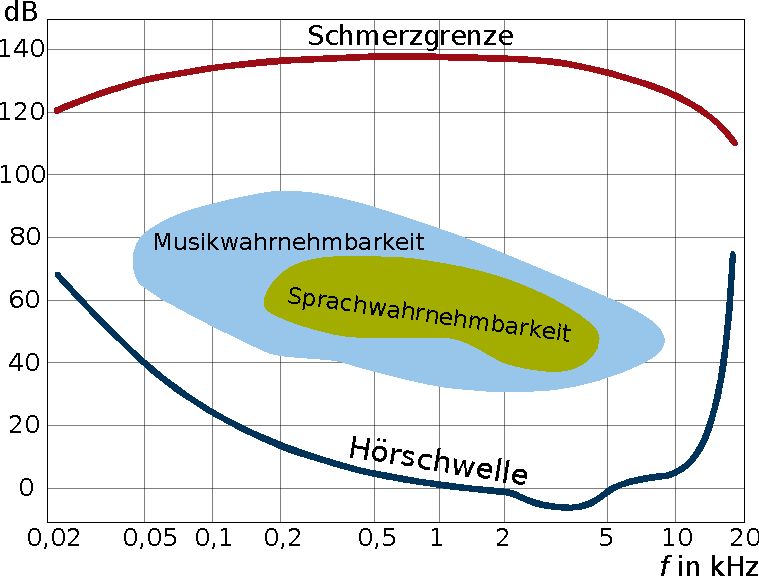
\includegraphics[width=\columnwidth]{./img/Hoerflaeche.pdf}
}

\sectionbox{
	\subsection{Wahrnehmung}
	Gehörganglänge: 2.5cm
	Tromelfell: $\SI{1}{\centi\meter\squared}$\\
	Schallintensität bei 90dB: $I = \SI{e-3}{\watt\per\meter\squared}$\\

	$IRT < \SI{85}{dB}$ \qquad $\hat L <\SI{130}{dB}$
	Kopfhörer: Kennschalpegel bei 1mW

	Tiefe Frequenzen: Weniger Gefährdung, deswegen nur 1 Picoloflöte aber viele (8) Kontrabässe.\\
	Schall-Leistung $L$: Faktor 2 entspricht 3dB\\
	Schalldruck $p$: Faktor 2 entspricht 6 dB\\
	Lautheit $S$: Faktor 2 entspricht 10 dB.\\
	\\
	Helmholz: Langzeitspektren zur Synthese:\\
	Klingt nicht authentisch, da einschwingvorgänge unberücksichtigt bleiben\\
}


\sectionbox{
\subsection{Schallpegelmesser Apps}
Noise Immission Analyzer (iPhone)
Noise Meter (Android)

Auflistung von EMPA.
}

\sectionbox{
\subsection{Kopfhörer}
Kennschalpegel: Schallpegel bei $\SI{1}{\milli\watt}$\\
Nennbelastbarkeit: Maximale Betriebsleistung\\
Klrirrfaktor: Verzerrung einer Eingangs-Sinusschwingung in \%\\


$\Delta L = 20 \lg \frac{U}{U_{\ir ref}} = 10 \lg \frac{P}{P_0}$ in $\si{dB}$\\
Maximaler Schaldruck: Kennschaldruck(dB) + $\Delta L$ bei Nennbelastbarkeit.
}


Frequenzunterschied hörbar bei 440 Hz: etwa 4 Hz
Kleine Unterschiede im Grundton sind schwer wahrnehmbar, mit harmonischen Obertönen 

\sectionbox{
\subsection{Vibrato}
Wichtige Größen: Geschwindigkeit und Exkursion ($\Delta f$)

Wahrnehmbare Unterschiede (Exkursion):\\
A2: 55 Cent, A3: 27 Cent, A6: 13 Cent\\
Deshalb Faktor 2 oder 3 für musikalisch gewollten Vibrato\\
Bei teifen Tönen langsam (3 Hz), bei hohen Tönen schnell (6 Hz)\\
}

\sectionbox{
	\subsection{Oktave}
	Bei einem Intervall nach oben fällt ein zu hoher Ton weniger auf als zu niedrig. Bei einem Intervall nach unten genau andersrum.\\
	Ein Stück klingt sogar besser, wenn die obere Stimme eine etwas größere Oktave zum Bass hat.
}






\sectionbox{
	\subsection{Lautheit}
	Lautheit (DIN45631): Lautstärke wird durch die Fläche des Frequenzspektrums bestimmt.
	4 sone werden doppelt so laut empfunden, wie 2 sone.
	IRT: Wie laut ist der Schall oder die Quelle? Man kann originalpegel an stimmen von bekannten personen erkennen. $\pm\SI{0.4}{dB}$
}


\sectionbox{
	\subsection{Virtuelle Tonhöhe}
	Die wahrgenommene Tonhöhe eines Klanges entspricht i.a. der Grundschwingung (1. Harmonische).
	Werden nur die höheren Obertöne übertragen und abgespielt, rechnet das Gehirn die niederen Obertöne bis zum Grundton zurück und fügt diese hinzu.
	Die wahrgenomme Tonhöhe bleibt damit gleich.\\
	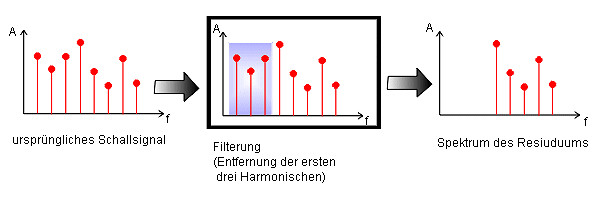
\includegraphics[width=\columnwidth]{./img/virtuelletonhoehe.jpg}
}


\sectionbox{
	\subsection{Psychoakustik}
	Die Psychoakustik befasst sich mit der subjektiven Wahrnehmung von Schall (Musik, Klang, Lärm etc.) und der Informations-Verarbeitung des Gehörs.
	Dabei werden eine Reihe akustischer Täuschungen beobachtet.\\

	\begin{description}
	\item[Shepard Pitch:] Ton der scheinbar unendlich nach oben oder nach unten verschoben wird.\\
		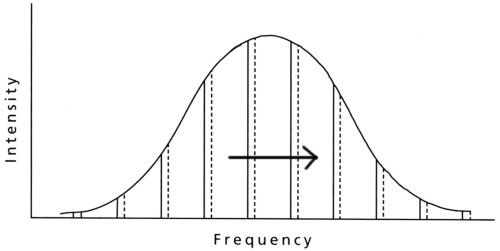
\includegraphics[width=0.8\columnwidth]{./img/shepard.jpg}
		Hüllkurve bleibt erhalten, die frequenzen werden zyklisch von einer seite zur anderen geschoben

	\item[Galloping Rhythm:] ein konstanter Ton mit abständen, dazwischen aufsteigender ton.\\
	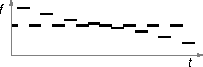
\includegraphics[width=0.8\columnwidth]{./img/galloping.pdf}\\
		Wenn sie sich treffen klingen sie gallopierend.\\


	\item[Continuity Effekt:] abwechselnd Musik (250ms) und weißes Rauschen (200ms) klingt kontinuierlich. Gehirn schätzt Verlauf\\
	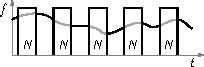
\includegraphics[width=0.8\columnwidth]{./img/continuity.pdf}

	\item[Remastering:] Wird hochfrequentes Rauschen von Platten entfernt, wirkt sich das negativ auf die Brillanz auf.
	Gewolltes hochfrequentes Rauschen damit Instrumente brillanter empfunden werden.


	\item[Tonhöhenverschiebung:]
	Bandbegrenztes Rauschen neben einem Ton verschiebt diesen im Frequenzspektrum von sich weg. Verschiebung nach oben im Mittel um 6\% nach unten um etwa 3 \%, allerdings ist dies personenabhängig.\\
	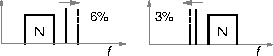
\includegraphics[width=0.9\columnwidth]{./img/tonhoehe.pdf}
	
	\item[Gesetz der 1. Wellenfront:] Kommt ein Peak von Links un der Rest vom Ton von rechts, dann hört man den kompletten Ton nur von link.
	
	
	\end{description}
}


% ##########################################################################
\section{Raum- und Bauakustik}
% ##########################################################################


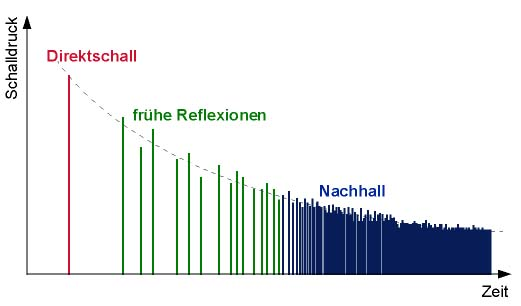
\includegraphics[width=\columnwidth]{./img/Akustik_Raumimpulsantwort.jpg}


\sectionbox{
	\subsection{Nachhallzeit}
	Zeitspanne, in welcher der Schalldruckpegel $L$ eines Schallereignisses ($\SI{1}{kHz}$) in einem Raum um $\Delta L_{\ir dB} = \SI{60}{dB}$ (auf $\frac{1}{1000}$) absinkt.
	Klagen über eine schlechte Akustik sind meistens mit nicht angemessenen Werten für die Nachhallzeit verknüpft.\\
	Grobe Richtwerte: Sprache $\le \SI{1}{s}$, Orchester 2s, Kirchenmusik 3...4s\\

	Messung: Breitbandiges Signal länger spielen und schlagartig aufhören.\\
	Sabinesche Nachhallformel: $T_{\ir N} = 0.163 \frac{V}{\ol \alpha S}$\\
	Absorbtionsfläche $S$, Mittlerer Absorptionskoeffizient $\ol \alpha$\\
	Äquivalente Absorbtionsfläche $A = \ol \alpha S\\$\\

	Messung:\\
	Schall um $-\SI{5}{dB}$ abfallen lassen und $T_{30}$ bis $-\SI{35}{dB}$ messen.\\
	$T_{60}$ nicht wegen Dynamikproblem, Hintegrundlärm\\
	\\
	Was tun gegen zu langes $T_{\ir N}$?\\
	Volumen reduzieren, abgehängte Decken, Raumteiler\\
	stärkere Absorbtionsflächen, jede Person ($\SI{0.5}{\meter\squared}$)


	\subsection{Hallradius}
	Abstand $r_{\ir H}$, bei dem Direktschallpegel $L_{\ir D}$ und Raumschallpegel $L_{\ir R}$ (frühe Reflexionen und Nachhall) gleich groß sind.\\ 
	$r_{\ir H} = 0.14 \sqrt{\ol \alpha S}$\\
	Gerichtetes Schallfeld: dominiert bis $r_{\ir H}$, danach dominiert diffuses Schallfeld\\
	$\ra$ Aufnahmen relativ nah am Instrument.\\
	Direct-to-reverberant ratio $DRR = \frac{E_{\ir gerichtet}}{E_{\ir diffus}}$
}


\sectionbox{
\subsection{Raumakustik}
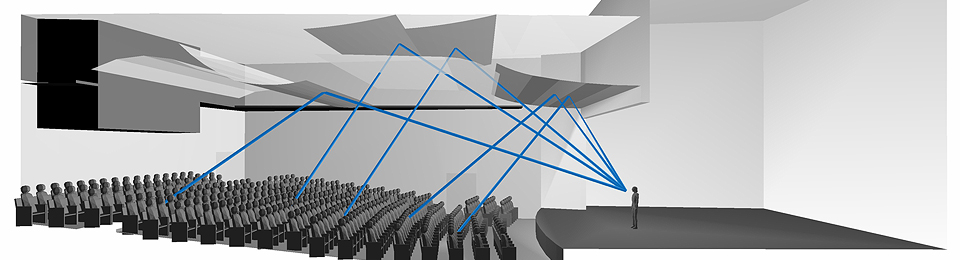
\includegraphics[width=\columnwidth]{./img/raumakustik.jpg}
\paragraph{Ziel:} Gut klingende Räume je nach Zweck.\\

\begin{description}
	\item[Studio:] Reflexionsarm, möglichst nur direkt Schall, keine Eigencharakteristik des Raumes, neutrale Wiedergabe.
	\item[Konzertsaal:] räumlicher und lebendiger Klang, viele frühe Reflexionen, Nachhallzeit 1 bis 3 Sekunden, Einhüllung
	\item[Konferenzraum:] Hohe Sprachverständlichkeit, Nachhallzeit $<$ 1 Sekunde, viel direkt Schall
\end{description}

	Viele Plätze (>2000) bedeutet viele Menschen, die Schall absorbieren.\\

	\subsubsection{Eigencharakteristik}
	Vivace: Mikro + Lautsprecher für künstliche Nachallzeit. Damit kann Konzersaalakustik im freien simuliert werden.\\
	IRCAM: Raum mit vielen verstellbaren Dreiecken die unterschiedliche Absorbtionskoeffizienten haben\\
	ATR: Drehbare Zylinder mit unterschiedlichen Absorbtionskoeffizienten.\\
	BR: Resonanzabsorber: Halboffene Kästen, die gedreht werden können.\\
}

\sectionbox{
	\subsection{Bauakustik}
	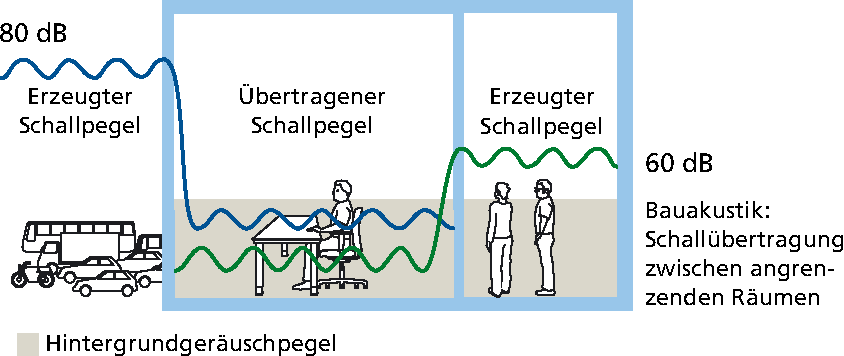
\includegraphics[width=\columnwidth]{./img/Bauakustik.pdf}
	\paragraph{Ziel:} Keine Störgeräusche im Raum. Es gibt Luftschallschutz und Trittschallschutz (Körperschall)\\
	Dämpfung von Wänden $\ol R = 13 \lg G + 15$\\
	Wandgewicht $G$ in $\si{\kilogram \per \meter\squared}$\\  

}





{\huge Exkursion:}\\

\sectionbox{
\subsection{Räume}


	
	\begin{description}
		\item[Runde Bauform:] (Kreis, Kupel) schlecht, viele Fokusierungen
		\item[Fächerform:] Mittel
		\item[Schuhschachtelform:] Gut, Frühe Reflexionen, breite Streuung des Schalls, keine Ausbildung von Brennpunkten wie bei Runden Bauformen.
		\item[Schräge Wände:] Verhinderung von stehenden Wellen, da es keine parallele Flächen gibt und dadruch reflektierte Wellen nicht in die gleiche Richtung zurücklaufen bzw. zwischen zwei Flächen gefangen werden.

		


		\item[Schallabsorber:] Feine Löcher und Schlitze in den Wänden/Flächen absorbieren den Schall und vermindern generell die Reflexion.
	\end{description}


}

\sectionbox{
\subsection{Mikrofone}

	\subsubsection{Intensitätsmikrophonie}
	Stereomikrophone an einem punktuellen Ort. Lautstärkeunterschiede bestimmen Position der Phantomschallquelle.


	\subsubsection{Laufzeitenmikrofonie}
	Mikrophonpärchen mit bestimmten Abstand. Laufzeitdifferenz zwischen Schallsignal bestimmt Position. \\
	Abstand vom Mikrofonpärchen:\\
	zu groß: Laufzeit zu groß, zu große Unterschiede im Klang, keine Phantomschallquelle mehr\\
	zu klein: weniger Stereoeffek, ungenauere Messung.\\

	
	\subsubsection{Polymikrophonie}
	Für jedes Instrument einzelnes Mikrophon, möglicherweise auch hintereinander aufgenommen.
	
	
	
	Kondensator (Druckempfänger): Neumann, Schöps\\
		Messmikrofon: Linearer Frequenzgang, dafür hohes Rauschen\\
	Dynamische (Schnelleempfänger): Senheise, Shure\\
		werden für Nahbesprechung
	Bändchen (Schnelleempfänger): Beyer\\
	\\
	
	
	
	\subsubsection{Charakteristika}
	Kugel, Acht, Niere, (Superniere, Hyperniere)\\

	\subsubsection{MS-Stereo}
	Mitte-Kanal $M$ (Kugelcharakteristik)\\
	Seite-Kanal $S$ (Achtcharakteristik)\\
	$M = L + R$ \qquad $S = L - R$\\
	$M+S = 2L$ \qquad $M-S=2R$\\
	
	\subsubsection{Koinzidenz-Mikrofone}
	2 verdrehbare Kondensatormikrofone
	
	Laufzeitenmikrofonie: Deccatree, Jecklin, ORTF\\
	Mikro testen: Mit Schlüsselbund klirren
}


\sectionbox{
	\subsection{Manger Schallwandler}
	\parbox{0.45\columnwidth}{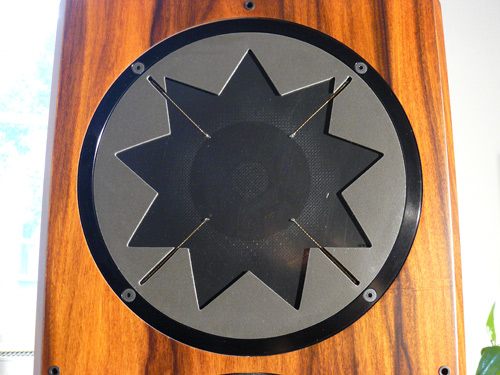
\includegraphics[width=0.4\columnwidth]{./img/manger-treiber.jpg}}
	\parbox{0.5\columnwidth}{
Das besondere am Manger Schallwandler ist, dass die Membran ausschließlich in sich selbst schwingt - so entstehen nämlich die mangertypischen "Biegewellen".
Der akustische Clou bei dem Ganzen ist, dass komplexe Schallsignale so phasengenau in ihre Komponenten zerlegt werden können.}
}


\sectionbox{
	\subsection{Musikaufnahme und Wiedergabe}
	Räumlichkeit für Pop-Rock: Niels Adelmann-Larsen\\
	Volumen und Nachhallzeit: 1,5 s gut, ab 3s schlecht.\\
	
}







% ##########################################################################
\section{Sonstiges}
% ##########################################################################

\sectionbox{
	\subsection{Akustische Begriffe:}
	\begin{description}
		\item[Schalldruck:] $p$ in Pa Druck der Schallwelle
		\item[Schallschnelle $v$:] Geschwindigkeit der sich bewegenden Teilchen
		\item[Schallgeschwindigkeit $c$:] Ausbreitungsgeschwindigkeit der Welle
		\item[Lautheit:] entspricht Menschlichem Lautstärkeempfinden. Einheit sone.
		\item[Kennschalldruck:]
		\item[Klirrfaktor:] Maß für unerwünschte Verzerrung eines Sinustons in \%.
		\item[Schallabsorptionsgrad:] $\alpha \in [0,1]$ Maß wie stark ein Material auftreffenden Schall absorbiert und in andere Energieform, z.B. Wärme umwandelt. 0 (totale Reflexion) und 1 (totale Absorbtion)


	\end{description}

}



\sectionbox{
	\subsection{Initial Time Delay Gap (ITDG)}
	Zeit $\Delta t$ zwischen dem zuerst eintreffenden Direktschall $D$ und den frühen Reflexionen $R$ des unkorrelierten Raumschalls.
	$\Delta t = \frac{(d_{R1} + d_{R2}) - d_D}{c}$

}

\sectionbox{
	\subsection{Wellenausbreitung}
	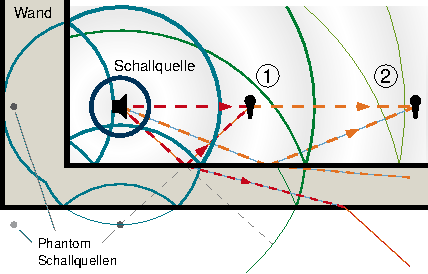
\includegraphics[width=\columnwidth]{./img/propagation.pdf}

	Reflektierte Wellen sehen so aus, als ob sie von einer Phantomschallquelle ausgehen, die den selben Abstand zur Fläche hat wie die Schallquelle selbst. (Vgl. Spiegelladungsmethode)
	Beim Mikrofon $\textcircled{\small 1}$ ist der Laufzeitunterschied zwischen Direktschall und erster Reflexion größer als bei $\textcircled{\small 2}$.
	In fester Materie(Wand) breitet sich Schall schneller aus, die Wellenfront wird sozusagen weggebrochen (Vlg. Optik). Ab einem bestimmten Einfallswinkel tritt Totalreflexion auf ($\textcircled{\small 2}$).

}

\sectionbox{
	\subsection{Reflexionen}
	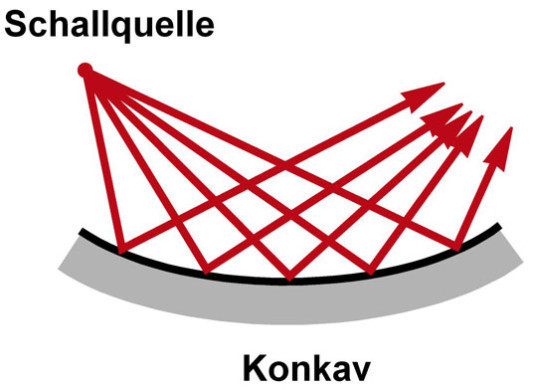
\includegraphics[width=0.5\columnwidth]{./img/ref_konkav.jpg} 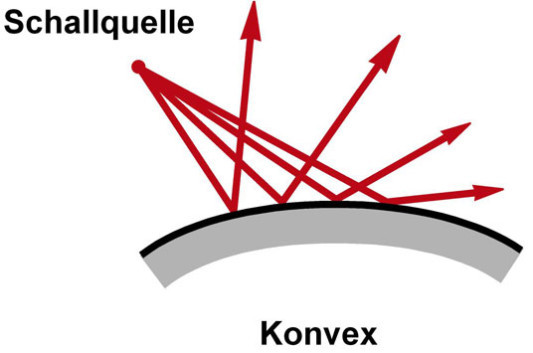
\includegraphics[width=0.5\columnwidth]{./img/ref_konvex.jpg} 


	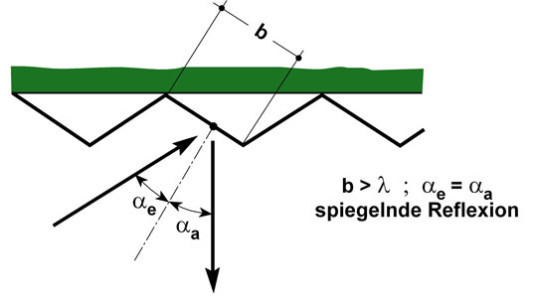
\includegraphics[width=0.8\columnwidth]{./img/ref_k.jpg}
	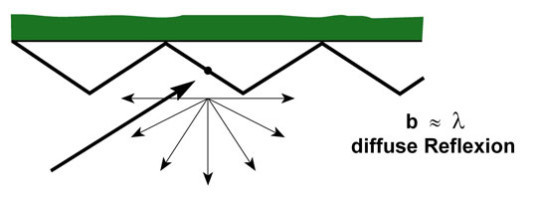
\includegraphics[width=0.8\columnwidth]{./img/ref_diffuse.jpg}
	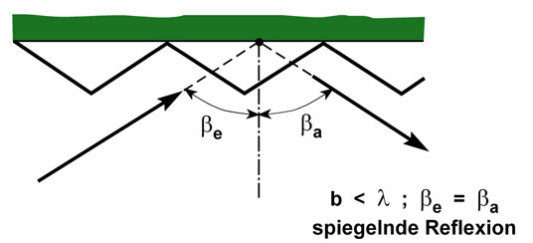
\includegraphics[width=0.8\columnwidth]{./img/ref_g.jpg}

}



\sectionbox{
	\subsection{Schallpegel}



	Addition: $L_1 + L_2 = 10 \log \left(10^\frac{L1}{10} + 10^\frac{L2}{10} \right)$
}

\sectionbox{
	\subsection{Raumresonanzen}
Raumresonanzen führen in Räumen zu einer Verschlechterung der Sprachverständlichkeit, da einzelne Frequenzen besonders hervorgehoben werden. 
Unter Raumresonanzen versteht man die Eigenfrequenzen der stehenden Wellen.\\
$f_{n_x,n_y,n_z} = \frac{c}{2} \cdot \sqrt{\left( \frac{n_x}{l_x} \right)^2 + \left( \frac{n_y}{l_y} \right)^2 + \left( \frac{n_z}{l_z} \right)^2}$\\
$n_x,n_y,n_z \in \N_0$

}

	\begin{tabular*}{\columnwidth}{@{\extracolsep\fill}llll@{}}
		\ctrule
		\multicolumn{2}{c}{\emph{Psychoakustik}} &\multicolumn{2}{c}{\emph{Physik}}\\
		Bezeichnung & Einheit & Bezeichnung & Einheit\\
		\cmrule
		Tonheit $Z$ &Bark& \multirow{2}{*}{ Frequenz $f$ }& \multirow{2}{*}{$Hz$}\\
		Verhältnistonh. $V$ & Mel & & \\
		& & Schalldruck $p$ & $\frac{N}{m^2} = Pa$\\
		& & Schallschnelle $v$ & $\frac{m}{s}$\\
		& & Schallintensität $I$ & $\frac{W}{m^2} = \frac{N}{s m}$\\
		Lautstrk.pegel $L_n$ & Phon & \multirow{2}{*}{Schalldruckp. $L$} &\multirow{2}{*}{ $dB$}\\
		Lautheit $N$ & sone\\
		& & Schallleist. $P_{ak}$ & $W = \frac{N m}{s}$\\
		\cmrule
		\multicolumn{4}{c}{Bezugsschalldruck $p_0 = 2\cdot 10^{-5} \frac{N}{m^2} = 20 \mu Pa$}\\
		\multicolumn{4}{c}{Bezugsintensität $I_0 = 1.0\cdot 10^{-12} \frac{W}{m^2}$}\\
		\cbrule
	\end{tabular*}



% #########################################################################################################
% #########################################################################################################
\newpage
% #########################################################################################################
% #########################################################################################################

% 2 Übungsstunden: Praktisch technische messung
% moodle: Helmholtz2015


% Prüfung: 18.02.15


{\huge \bfseries Technische Akustik}\\[0.5em]


\emphbox{ \textbf{HINWEIS}: Die Formelsammlung ist bisher noch eine einfache Mitschrift, teilweise
ungeordnet und kann grobe Fehler enthalten. }


\sectionbox{
	\subsection{Was ist Lärm}
	Disco, Kegelbahn, Flugzeug, Motorrad\\
	Die Beurteilung macht den Schall zum Lärm. Unerwünschte Schallereignisse.\\
	\\
	Berufskrankheiten: Haut, Schwerhörigkeit\\
	Lärm macht krank: Kommunikationsstörung, Adrenalin, Schlafstörung, Bluthochdruck, Stress\\
	Sound Quality Design: Active Noise Cancelation: Motorgeräusche weniger, Windgeräusche aufdringlicher?\\
}

\sectionbox{
	\subsection{Belästigung}
	Durch Lärm gestört oder belästigt:\\
	3000 Luete, Hausbesuch, Telefon:\\
		\begin{tabular}{lccc}
		& Stark & Mittel & Etwas\\ \mrule
		Straße & 6\% & 20\% & 28\%\\
		Nachbarn & 3\% & 14\% & 25\%\\
		Schiene & 3\% & 12\% & 19\%\\
		Industrie & 2\% & 4\% & 19\%\\
		Flugverkehr & 1\% & 5\% 17\%\\
		\end{tabular}
	
	Online Umfrage:\\
	\begin{tabular}{lll}
		& stark & mittel\\
	Straße & 36\% & 59\%\\
	Nachbarn & 18\% & 32\%\\
	Fluglärm & 20\% & 30\%\\
	\end{tabular}
}

\sectionbox{
	\subsection{Maßnahmen}
	Asphalt statt Kopfsteinplaster\\
	Geschwindigkeitsbegrenzung\\
	Schallschutzwände\\
	Tunnel\\
	Nachtfahrverbote\\
	Verkehrsbündelung: Einbahnstraßen\\
	\\
	Fahrer:\\
	50 kmh: 2.Gang vs 3.Gang: 6dB leiser!\\
	\\
	Fluglärm:\\
	Mantelstromtriebwerke: 20dB leiser (vs. Düsenjäger)\\
	Möglichst steil starten und landen (höherer verbrauch)\\
	Nachtflugverbot\\
	\\
	Schienenlärm\\
}

\sectionbox{
	\subsection{Systemtheoretischen Ansatz}
	Schallwellen mit Impedanz\\
	Impedanzanpassung für möglichst schlechte Leistungsübertragung (maximale Reflexion)\\

	\subsection{Lärmbekämpfung Schallquelle}
	Elektro- statt Verbrennungsmotor\\
	Veringerung der Drehzahl\\
	Fallhöhe verringern\\
	Keine scharfen Winkel bei Wasserrohren\\

	\subsection{Schallübertragung}
	Federnde Lagerung von virbierenden Maschinen\\
	Rohre mit Schallweichen Material befestigen\\
	Schwimmender Estrich um Trittschall zu minimieren\\
	Doppelhaus, Spalte dazwischen (Mörtelklumpen stellt Schallbrücke her)\\
	
	\subsection{Schallabstrahlung}
	Fläche reduzieren\\
	Gußteile (Vacrosil)\\
	Entdröhnbeläge\\
	
	\subsection{Schallausbreitung}
	am Entstehungsort\\
	Umschließen (Box) mit innen Dämmmaterial (Steinwolle) und außen Entdröhnbeläge\\
	Gehörtschützer\\ 
	Watte/Taschentuch 10...20dB\\
	Stöpsel (lin. Freq.) 10...30dB\\
	Kapsel 15...40dB\\
	Helm 15...50dB\\
	Undichte Fenster ...25dB\\
	Isolierglass ...35dB\\
	Schallschutzfenster ...45dB\\



}

\sectionbox{
	\subsection{Active Noise Canceling (ANC)}
	Lüftungsgeräusche ...60dB\\
	BMW ...10dB\\

}

\sectionbox{
	\subsection{Schallfeldgrößen}
	
	\subsubsection{Particle velocity (Schallschnelle)}
	Bewegungsgeschwindigkeit eines Teilchens, durch Kopplung ist Schallgeschwindigkeit höher
	$v = \frac{\diff \vec s}{\diff t}$\\
	typ. Werte: $\num{e-8}...\SI{e-2}{\meter\per\second}$\\
	\\
	\subsubsection{Speed of sound (Schallgeschwindigkeit) $c$}
	Ausbreitungungsgeschwindigkeit der Welle\\
	$c = 331.5 + 0.6 \frac{T}{\si{\celsius}} \si{\meter\per\second}$
	
	\subsection{Abgeleitete Größen}
	DIN EN ISO 80000-8 und DEGA Empfehlung 101\\
	
	\begin{tabular*}{\columnwidth}{@{\extracolsep\fill}lll@{}} \ctrule
		Größe & Formel & Einheit\\ \cmrule
		Schallenergieflussdichte & $\vec i = p \vec v$ & $\si{\watt\per\meter\squared}$\\
		Schallintensität & $I=\frac{1}{t_2 - t_1} \int_{t_1}^{t_2} i(t) \diff t$ & $\si{\watt\per\meter\squared}$\\
			& $I = p \cdot v$ & \\
		Schallleistung & $P = I \cdot S$ & $\si{\watt}$\\
		spez. Schallfeldimpedanz & $Z_{\ir S} = \frac{p}{v} = \frac{F}{S \cdot v}$ & $\si{\newton\second\per\meter\cubed}$\\
		Mechanische Impedanz &  $Z_{\ir m} = \frac{F}{v} = Z_{\ir s} \cdot S$ & $\si{\newton\second\per\meter}$\\
		Schalldruckpegel & $L_{\ir p} = 20 \log \frac{p}{p_0}$ & $\si{dB}$\\
		Schallintensitätspegel & $L_{\ir I} = 10 \log\frac{I}{I_0}$ & $\si{dB}$\\
		Schallleistungsspegel & $L_{\ir W} = 10 \log\frac{P}{P_0}$ & $\si{dB}$\\
		
		\cbrule
	\end{tabular*}

	Bezugspegel $p_0 = \SI{20}{\micro\pascal}$ \qquad $I_0 = \SI{e-12}{\watt\per\meter\squared}$ \qquad $P_0 = \SI{e-12}{\watt}$

}

\sectionbox{
	\subsection{}
	Faktor: $p,v$ (Grundgrößen) \qquad Grad: $I,P$ (Energiegrößen)\\

	Beispiel: Reflexionsfaktor 0,1 entspricht Reflexionsgrad 0,01!\\

	\begin{tabular}{rrr} \ctrule
		$I/I_0$ bzw. $P/P_0$ & $L$ & $p,v$\\ \cmrule
		1 & $\SI{0}{dB}$ & 1\\
2 & $\approx \SI{3}{dB}$ & $\sqrt{2}$\\
4 & $\approx \SI{6}{dB}$ & 2\\
10 & $\SI{10}{dB}$ & $\sqrt{10}$\\
25 & $\approx \SI{14}{dB}$ & $5$\\
100 & $\SI{20}{dB}$ & 20\\
1000 & $\SI{30}{dB}$ & $\approx 31.6$\\
10000 & $\SI{40}{dB}$ & 100\\ \cbrule
	\end{tabular}
}

\sectionbox{
	\subsection{Addition von Geräuschen}
	Industrie: $L_{p1} = \SI{76}{dB}$\\
	Rasenmäher: $L_{p2} = \SI{70}{dB}$\\
	\subsubsection{Kohärente Schalle}
	Druckaddition. gleiches $f,\varphi$: doppelter Druck\\
	$L = 20 \log_{10} \left(10^{\frac{L_1}{20}} + 10^{\frac{L_2}{20}}\right)$
	\subsubsection{Inkohärente Schalle}
	zufällige Phasen und Pegel.
	Addition der Schallintensitäten.\\
	$I_1 = I_0 \cdot 10^{\frac{76}{10}}$ \qquad $I_2 = I_0 \cdot 10^{\frac{70}{10}}$\\
	$I = I_1 + I_2 = I_0 \cdot \left( 10^{\frac{76}{10}} + 10^{\frac{70}{10}} \right) = I_0 \cdot 10^{\frac{77}{10}}$\\
	Ab $\ge \SI{10}{dB}$ Unterschied, keine Auswirkung.\\
	$\SI{6}{dB}$ Unterschied, $\SI{1}{dB}$ dazu.\\
	Gleiche Pegel: $\SI{3}{dB}$ dazu. 
}

\sectionbox{
	\subsection{Tonabnehmer}
	
	Druckempfänger: Kondensatormikrofon: Lusftschlitz für statischen Druckausgleich, bestimmt die Grenzfrequenz. Je kleiner, desto tiefer die Grenzfrequenz.\\
	Schnelleempfänger: Bänchenmikrofon\\
	Intensitätsmeßsonde: $I = p \cdot v$\\
	2 Druckmikrofone, einmal Differenzschall ($v$), einmal Additionsdruck ($p$)\\
	Wellengleichung: $-\grad p = \varrho_0 \frac{\diff \vec v}{\diff t}$\\
}


\section{Entstehung und Ausbreitung}
\sectionbox{
	\subsection{Einfache Schwinger}
	
	\begin{tabular}{lll}
	Art & Beispiel & Medium\\
	Longitudinal & Dichtewelle & Gas, flüssig, fest\\
	Transversal & Saite & Biegeweiches Material\\
	Biegewelle & & Dünne Bleche\\
	Torsionswelle & Drehwelle & Stäbe\\
	\end{tabular}
	Transversal schneller als Longitudinal

}

\sectionbox{
	\subsection{Schallfelder}
	Elastizitätsgesetz $p(t) = c^2 \varrho(t)$ bzw. $\Delta p = c^2 Δϱ$\\
	Bewegungsgesetz: $-\grad p = \varrho \frac{\diff \vec v}{\diff t}$\\
	Kontinuitätsgleichung: $ϱ_0 \div \vec v = - \frac{\partial ϱ}{\partial t}$\\
	Wellengleichung: $\underbrace{\laplace}{\div \grad} p = \frac{1}{c^2} \frac{\partial^2 p}{\partial t^2}$\\
	Allg. Kompressionsgesetz: $\div \vec v = - \frac{1}{\rho_0 c^2} \frac{\partial p}{\partial t}$
}

\sectionbox{
	\subsection{Wellenausbreitung}
	
	Reflektoren: Wellenwiderstandsprung\\
	Luft: polierter Marmor (härter), Wasser: Schaumstoff (weicher)\\
	
		\subsubsection{Ebene Wellen}
		$p$ und $v$ in Phase.\\
		$Z_s = \frac{p(x,t)}{v(x,t)} = ϱ \cdot c = Z_0$ \qquad reell bei ebenen Wellen
		Luft: $Z_0 = \SI{1,2}{\kilo\gram\per\meter\cubed} \cdot \SI{344}{\meter\per\second} = \SI{416}{\newton \second \per \meter\cubed}$\\
		Wasser: $Z_0 = \SI{1000}{\kilo\gram\per\meter\cubed} \cdot \SI{1.5}{\kilo\meter\per\second} = \SI{1.5e6}{\newton \second \per \meter\cubed}$\\
		
		\subsubsection{Kugelwellen}
		$Z_S = ϱ \cdot c\frac{2π\j \frac{r}{λ}}{1 + 2π\j \frac{r}{λ}}$\\
		Wellenzahl $k = \frac{ω}{c} = \frac{2π}{λ}$\\
		Mit Entfernung zum Sender: Übergang von Kugelwelle(Nahfeld) zur ebenen Welle (Fernfeld)\\

		Wann strahlt ein Lautsprecher Kugelwellen ab: Radius der Box $R$. Fernfeld ab $λ > 2π R$\\
		
		Versuch: Lautsprecher (10cm), 400Hz 4000Hz\\
		400Hz: Kugelwellen ($ΔL = \SI{3}{dB}$), 4000Hz: Gerichtet ($ΔL = \SI{11}{dB}$)\\ 
		\subsubsection{Stehende Wellen}
}

\sectionbox{
	\subsection{Strahlerarten}
	Punktstrahler: $p = \frac{r_0}{r} p_0$\\
	Bedingung für Kugelwelle: $r \gg λ, r \gg d,l$\\
	
	\subsubsection{Punktstrahler}
	$-\SI{6}{dB}$ pro Verdopplung von $r$\\
	

	\subsubsection{Linienquelle (Zylinderquelle)}
	Ausbreitung in 2 Dimensionen.\\
	$-\SI{3}{dB}$ pro Verdopplung von $r$\\
	Beispiel: Autobahn, Güterzug
	
	\subsubsection{Flächenstrahler}
	Keine Abnahme bei vergrößerung der Entfernung, wenn unendlich ausgedehnt.
	z.B. Bürogebäude mit schwingenden Fenstern
	
}

\sectionbox{
	\subsection{Resonatoren}
	$\frac{λ}{4}$-Resonator: $f = \frac{c}{l} \left( \frac14 + n \frac12 \right)$\\
	$\frac{λ}{2}$-Resonator: $f = \frac{c}{l} \left( \frac12 + n \frac12 \right)$\\	
}

\sectionbox{
	\subsection{Helmholtz-Resonator}
	Ein Helmholtz-Resonator besteht aus einem Luftvolumen in beliebiger Form, das einen zylindrischen engeren kurzen Hals mit einer Öffnung nach außen besitzt.
	$$f = \frac{c}{2π} \sqrt{\frac{S_{\ir Offnung}}{V_{\ir Bauch} \left(l_{\ir Hals} \cdot \frac{π}{2} \cdot r_{\ir Hals} \right)}}$$
}

\sectionbox{
	\subsection{Reflektierte Welle}
	Winkel $α$\\
	$p_{\ir in} (x,y,t) = p_0 \exp(\j(ωt - kx \cos α - ky \sin α))$\\
	$p_{\ir ref} (x,y,t) = p_0 r \exp(\j(ωt + kx \cos α - ky \sin α))$\\
	
	Reflexionsfaktor $r = \frac{p_{\ir ref}}{p_{\ir in}} = \frac{Z \cos α - Z_0}{Z \cos α + Z_0}$\\
	
	\subsection{Absorbierte Welle}
	Absorbtionsgrad $α = \frac{\abs{p_{\ir in}}^2 - \abs{p_{\ir ref}}^2}{\abs{p_{\ir in}}^2} = 1 - \abs{r}^2$\\
}


\sectionbox{
    \subsection{Plattenresonator}
    $f = \frac{c}{2π} \sqrt{\frac{ρ_{\ir Luft}}{ρ_{\ir Platte} \cdot D \cdot d}}$\\
	$Z = w'' + \j(ωm'' - \frac{Z_0}{ωd})$
}


\sectionbox{
    \subsection{Schallwellen}
    1D: $p(x,t) = p_0 \cos\left(\omega t + k x\right) = p_0 \cos\left(2π (ft + λx)\right)$
    
    
    \subsubsection{Reflexion/Absorbtion}
	Beispiel: Wandteppich im Abstand $\frac{λ}{4}$ zur Wand ($v = \max$) zur Dämpfung\\
	Akustikplatten mit Abstand von der Wand (dämpft tiefere Frequenzen, günstiger)\\

	\subsubsection{Brechung}
	Snellius'sche Brechungsgesetz: $\frac{\sin α}{\sin β} = \frac{c_1}{c_2}$\\
	Normalwetterlage: Oben kälter als unten, Schallgeschwindigkeit unten höher\\
	Positiv bei Flugzeugen: Brechung weg vom Boden, erzeugt Schattenzonen\\
	Bei Inversionswetterlage umgekehrt.\\
	Wind: In Windrichtung höhere Pegel.\\
	
	\subsubsection{Streuung}
	Raue Oberfläche: geometrische Reflexion an der ideal glatten Wand mit $(1-α)(1-s)$ + Streuung mit $(1-α)s$\\
	Streukoeffizient $s = 1 - \frac{E_{\ir geo}}{E_{\ir ges}}$


	\subsubsection{Beugung}
	Wellen werden an einem Hinderniss (z.B Kante) abgelenkt.
	Schallschutzwand: Beugung oben drüber mit Zusatzweg $d$.
	Dämpfung $ΔL \approx 10 \lg \left(2π^2 \frac{d}{λ}\right)$
}


\sectionbox{
    \subsection{3D Wellenfeld}
	In einem Quaderförmigen Raum.
	$p(x,y,z) = \sum\limits_{n_x = 0}^\infty \sum\limits_{n_y = 0}^\infty \sum\limits_{n_z = 0}^\infty p_0 \cos\left(\frac{n_x π x}{l_x}\right) \cos\left(\frac{n_y π y}{l_y}\right) \cos\left(\frac{n_z π z}{l_z}\right)$

	Resonanzen: $f_{n_x,n_y,n_z} = \frac{c}{2} \cdot \sqrt{\left( \frac{n_x}{l_x} \right)^2 + \left( \frac{n_y}{l_y} \right)^2 + \left( \frac{n_z}{l_z} \right)^2}$\\
$n_x,n_y,n_z \in \N_0$
}

\sectionbox{
    \subsection{Raummoden (Eigenfrequenzen des Raums)}
	Formant Frequenz: $M(f) \approx \frac{4π}{3} \left(\frac{f}{c}\right)^3 \cdot V$\\
	Beispiel: Hörsaal mit $7 \cdot 10 \cdot 2.8 = \SI{200}{\centi\meter\cubed}$ hat 880 Raummoden bis zur ersten Formantfrequenz bei $\SI{350}{Hz}$\\
	
	Raummodendichte: $\frac{ΔM}{Δf}$: Im Beispielraum bei $f=\SI{1}{\kilo\hertz}$ bereits 62 Resonanzfrequenzen bei $\SI{1}{Hz}$ Bandbreite.\\
	Für akustischen Messungen sollte $\frac{ΔM}{Δf} \ge \frac{1}{\si{Hz}}$\\
	Für Beispielraum $f \stackrel{!}{>} \SI{125}{Hz}$\\
	Genauer Schröder Frequenz\\
	
	\subsubsection{Schröder Frequenz}
	$f_{\ir S} \gg 2100 \sqrt{\frac{T_{60}}{V}}$\\ 

	\subsubsection{Mittlere Reflexionsrate}
	Mittlere Reflexionsrate $\ol n = \frac{cS}{nV}$ in $\si{\per\second}$\\
	Mittlere freie Weglänge $\ol l = \frac{4V}{S}$ in $\si{\meter}$
}

\sectionbox{
    \subsection{Statistische Raumakustik}
    Wellentheorie: wenig Hindernisse\\
    Strahlen: $\lambda < L_{x,y,z}$ der Hindernisse.\\
    Energie: gleichmäßige Verteilung der Energie.\\
	\\
	Nachhallzeit $T_{60}$

}

\sectionbox{
    \subsection{Nachhallzeit}
Abklingen nach $n$ Reflexionen: $E(t) \approx E_0 (1- \ol{α})^{\ol n t} = E_0 \exp(\ol n t \ln(1-\ol{α}))$\\
$L(t) = L_0 \frac{10}{\ln (10)} \ol n t \ln(1-\ol{α}) = L_0 4,34 \ol n t \ln(1-\ol{α})$\\
$T_{\ir N} = - \frac{60}{4,34 \ol{n} \ln(1-\ol{α})}$
$T_N = -\frac{24 \ln(10)}{c} \cdot \frac{V}{S - \ln(1-\ol \alpha)}$
}

\sectionbox{
    \subsection{Raumsimulationstechniken}
    Spiegelschallquellenmethode: an Reflexionsflächen\\
    Raytracing: Strahlen in alle Richtungen\\
    Finite Elemente: Bewegung an Begrenzungsflächen\\

}

\sectionbox{
    \subsection{Perzeptive Aspekte in Räumen}
    
    \subsubsection{Präzidenzeffekt}
    % Gesetz der ersten Wellenfront, Lokalisationsdominanz
    Korrekte Lokalisation und Fusion mit den Reflexionen des Direktschalls trotz stärkerem diffusen Schallfeld

	\subsubsection{Haas-Effekt}
	Sprachunverständlichkeit gestört, wenn Reflexionen bestimmte Schwelle überschreiten (Pegel, Laufzeit)
	
	\subsubsection{Clarity / Klarheitsmaß}
	$C_{50} = 10 \log \frac{\int_0^{50} p^2(t) \diff t}{\int_{50}^\infty p^2 (t)\diff t}$ \qquad $\SI{80}{\milli\second}$ für Musik\\
	ISO 3382\\
	
	\subsubsection{Speach Transmission Index(STI)}
	Bewertung: Moduliertes Signal im Raum: Wie stark wird die Modulationstiefe verringert?\\
	$I_i(1+m_i \cos(2πft))$ wird zu $I_0(1+m_0 \cos(2πft)$\\
	Modulationstranferfunktion(MTF) $m=\frac{m_0}{m_i}$\\
	MTF wird mit Testsignal bestimmt(Okavbänder, SNR)\\
	SNR pro Oktavband spektral gewichtet ergibt Sprachverständlichkeit $STI \in[0; 1]$\\
	
}


\sectionbox{
    \subsection{Schalldämmung}
	Reflexionsgrad $ϱ = (1-α)$\\
	Absorbtionsgrad $α = δ + τ$\\
	Dissipationsgrad $δ$\\
	Transmissionsgrad $τ = 1-(ϱ + δ)$\\
	
	$R_g = 10\lg \frac{1}{τ}$\\
	Luftschalldämmmaß: 100Hz: 33dB; 1,6kHz: 56dB
}

\sectionbox{
    \subsection{Koinzident Effekt}
    Schwingende Trennwand, Biegewelle "Spuranpassung".\\
    Wenn die Schallwelle die Wand mit Resonanzfrequenz anregt, dann hat sie theoretisch keine Dämmung.\\
	\\
	\subsubsection{Was kann man tun?}
	1. Doppeltes Wandgewicht: nur 4dB weniger\\
	2. viele Wellenwiderstandssprünge: theoretisch doppelte Dämmung\\
	Entkopplung nötig, seperate Aufständerung, mechanisch empfindlich\\
	Dämmung der zweischaligen Konstruktion kann bis zum 35-fachen Wandgewicht der einschaligen Konstruktion entsprechen!\\
	3. Abstand erhöhen und Dämmaterial im eigenen Raum: veringert diffuses Schallfeld und erhöht Hallradius.\\ 

	\subsubsection{Demo: Zwei angrenzende Kästen}
	Im Empfangsraum ohne Wand: 100dB(A)\\
	Wand1: $\SI{809}{\gram\per\meter\squared}$ \qquad gerechnet: $\ol R = 13,7dB$\\
	gemessen: 85dB\\
	Wand2: $\SI{1900}{\gram\per\meter\squared}$ \qquad gerechnet: $\ol R = 18,6dB$\\
	gemessen: 80dB\\
	Mit Absorber im Empfangsraum: 62dB\\
	Mit Absorber im Senderaum: 56dB\\
}

\sectionbox{
    \subsection{Körperschalldämmung}
	Trittschall: direkte Abstrahlung und Einkopplung ins Material.\\
	Lösung: Schwimmender Estrich: Beton, Gummimatte, Beton(entkoppelt)\\
	Messung(Norm): Hammerwerk aus 5 Hämmer mit 500g

	$L_n = L_{\ir Terz} - 10\lg \frac{\SI{10}{\meter\squared}}{\ol \alpha S}$
	
	Demo: Hammerwerk auf Decke: 100dB(A)\\
	auf Stragula: 95dB(A)\\
	Schaumstoff+Sperrholz: 86dB(A)\\
	mit Schallbrücke: 93dB(A)\\
}

\sectionbox{
    \subsection{}
	RMS = $\sqrt{\frac{1}{N} \sum (p[n])^2}$

	A-Bewertung: Pegelanpassung nach Isophonkurve bei 40dB (Hörfläche)\\ 
	A-Filter\\
}

\sectionbox{
    \subsection{Zeitkonstante}
	Gehör: Töne von 10ms auf 100ms verlängert: doppelte Lautheit!\\
	Keine Lautstärke Zunahme oberhalb 200ms\\
	Zeitkonstante $I = \SI{35}{ms}$ wie "impulse"\\ 
	Zeitkonstante $F = \SI{125}{ms}$ wie "fast"\\ 
	Zeitkonstante $S = \SI{1}{s}$ wie "slow"\\ 
}

\sectionbox{
    \subsection{Drehkörper}
    Hellikopter, Ventilator\\
    Bei stationären Schallen einfach, bei impulshaften Schallen tradeoff:
    Unschärfe bei DFT $Δf \cdot T_{ein} = 1$
	Bei 200ms Schall, 5Hz Auflösung\\
	
	Mehr Lüfterblätter oder größere Fläche, reduziert Lärm.\\
	Demo:\\
	4 Flügel, 3000upm, $L_{AS} = \SI{86,4}{dB}(A)$\\
	16 Flügel, 750upm, $L_{AS} = \SI{56,5}{dB}(A)$\\
}

\sectionbox{
    \subsection{}
	Rosa Rauschen: $L_{ges} = L_{Terz} + \SI{15}{dB}$\\
	$k=\SI{15}{dB} - α$\\
	
	%fm		LTerz	Lterz-LA	k			De
	%100		40		-15dB		15-19=-4	-19
	%1000	60		+5			15-0=15		+20
	%2000	60		+5			15-(-1)=16	+21		
	%200000	20		-35			15-10+5		-30

	Einfügungsdämmaß:\\
	$D_e = (L_{\ir Terz} - L_{\ir A}) + k$\\
	Um wie viel muss der Pegel abgesenkt werden?
}

\sectionbox{
    \subsection{Lautheit}
    $N = 2^{\frac{L_N - 40}{10}} \quad [sone]$\\
    
	Lautheit: 1 sone ist 40dB bei 1kHz\\
	+10 dB verdoppelt sone\\	
	Bei gleichem dB(A) Wert ist breitbandiger Schall lauter als schmalbandiger Schall. (Bis Faktor 3)\\

	\subsubsection{Lautstärkepegel in Phone}
	Zum Vergleich: Lautstärkepegel $L_N$ in phone (equivalenter 1kHz Sinston, der genau so laut ist wie der zu bestimmende Schall)\\
	Achtung: bei niedrigen phone nicht linearer Zusammenhang: Von 9 auf 11 phone entspricht Verdopplung der Lautstärke.\\ 

		\subsubsection{Zwicker-Lautheit}
	Terzbänder: $B = 0.23 \cdot f_{\ir m}$ als Bandbreite\\
	Gehörfilter: $B = 100Hz$ bei $f_m < \SI{500}{Hz}$ und $0.2 f_m$ bei $f_m > \SI{500}{Hz}$\\
	Empfindlichkeit unterschiedlich bei verschiedenen Mittenfrequenzen $f_m$\\
	Tiefere Frequenzen können höhere verdecken $\ra$ Maskierung\\

	Im Diagram ist die Fläche proportional zur wahrgenpommenen Lautheit\\
	Demo: Lautheit eines Küchenmixers\\
	1. Messung Frequenzspektrum\\
	2. trage Terzpegel ein, über 280Hz direkt, unter 280Hz fasse Pegel zusammen.\\
	% 31.5Hz	42.9dB
	% 40Hz		33.8
	% 50Hz		35.0dB
	% 63Hz		33.9dB
	% 80Hz		36.0	
	% 100Hz		35.3
	% 125Hz		35.0
	% 160Hz		37.2
	% 200Hz		39.8
	% 250Hz		43.6
	3. Verbinden: Aufsteigende Pegel senkrecht direkt, absteigende parallel zur Mithörschwellen
	4. Integriere Fläche, und ermittle Mittelwert: Lautheit

	\subsubsection{Psychoakustische Lästigkeit}
	Abhängig vom Bezug zur Quelle. Natürliche Geräusche weniger läsig als künstliche.
	Meist lästig, wenn hohe Frequenzen und periodischer Schall.\\
	Abhängig von Lautheit $N$,\\ 
	Schärfe $S$ (z.B. Zischen),\\
	Schwankungsstärke $F$ (z.B. Sirene),\\
	Rauigkeit $R$ (z.B Trillerpfeife),\\
	Ausgeprägtheit der Tonhöhe $ATH$ (z.B. Lüfter),\\ 			% Wie stark sind harmonische ausgeprägt


	
	

}

% Audioanlagen für rosa rauschen ausgelegt: weißes rauschen beansprucht hochtöner stärker



\sectionbox{
	\subsection{Sprachverständlichkeit}
	Speech Interference Level $SIL$			
	Wichtige Frequenzen: einge kHz bei Vokale, hohe Freq. für Konsonanten.\\
	Konsonanten wichtiger für Wortverständlichkeit.\\
	50\% Wortverständlichket liefert häufig 100\% Satzverständlichkeit allerdings mit sehr hoher Anstrengung.\\
	
		\subsubsection{Messung}
		Reintest: Konsonantentest\\
		Sotschek: Forced Choice: Markieren Sie das Wort: hin, drin, bin, Sinn\\
		Hagermann Matrixtest: Alles hat 10 Ausprägungen, Satz: Name--Verb--Zahl--adjektiv--Objekt\\  
}

\sectionbox{
    \subsection{Hörschwellenverschiebung}
    TTS: temporary threshold shift\\
    Beispiel: 8h Arbeitslärm, danach 16h zum abklingen der TTS.
    Falls TTS nicht abklingen kann summieren sich mehrere auf und es folgt eine
    PTS: permanent threshold shift.\\
    Im Alter von 30 bis 70 Jahre: 10dB Verlust durch absterben von Härchen.\\
    Grund: Altererscheinung, angesammelte PTS, kognitive Einschränkungen, genetische Prädisposition.\\
		
		\subsubsection{Ursachen}
		Einzelereignisse: Silvesterkracher (Empfehlung $<\SI{130}{dB}$)\\
		Spitzenpegel sind schwer zu messen, da integriert wird\\
		
		Langzeitgeräusche: Über 8h Arbeitstag gemittelt. 8h 85dB(A) entspricht 4h 88dB(A)\\
    
    Ab 85dB(A) muss ein vom Arbeitgeber gestellter Gehörschutz verwendet werden.\\
		% Morgen 17:00 HS: 2300
    
		\subsubsection{Messung}
		Für mehrere Stunden wiederholen:\\
		Für 22min dem Lärm aussetzen, 8min Pause und Hörschwelle bestimmen.\\
		Bei Sättigung (4-6 Stunden): Asmptotic threshold shift (ATS)\\
		Ab 75dB Geräusch steigt ATS mit 1,7dB mehr ATS pro 1dB Geräusch\\
	
		
}


\sectionbox{
    \subsection{Schallabwehr, Vorschriften, Normen}
    DIN, ISO, VDI-Richtlinien, ITG, DEGA, ASA
    
		\subsubsection{Arbeitslärm}
		Falls Pegel $L_{\ir A} > \SI{85}{dB(A)}$ bei Mittelung über 8h\\
		oder $L_{\ir C,Peak} > \SI{137}{dB(C)}$ muss der Arbeitgeber den Arbeitnehmer zum Tragen eines Gehörschutzes zwingen.\\
		\\
		Bei $L_{\ir A} > \SI{80}{dB(A)}$ oder $L_{\ir C,Peak} > \SI{135}{dB(C)}$ muss Gehörschutz zur Verfügung gestellt werden.\\

		\subsubsection{Maschinenlärm}
		Baumaschinen: in 7m Abstand $L_A < \SI{75}{dB(A)}$\\
		Rasenmäher: $L_{W,A} \le \SI{88}{dB(A)}$, auch von 19-22h benutzbar\\
			erkennbar an dem „blauen Umweltengel“\\
		
		Was sind $\SI{90}{dB}$ Leistungspegel?\\
		$P= I \cdot S$, $L_W = 10 \log \frac{P_A}{P_0} dB$ \quad $P_0 = \SI{e-12}{W}$\\
		$P_A = 10^{\frac{90}{10}} \cdot \SI{e-12}{W} =\SI{e-3}{W}$\\
		In 10m Abstand?\\
		$S = 4πr^2 = 4 \cdot π 100m^2 \approx 1200m^2$\\
		$I_{A,10m} \approx \frac{\SI{e-3}{W}}{\SI{e3}{m^2}} = \SI{e-6}{\watt\per\meter\squared}$\\ 
		$L_{A,10m} = 10 \log \frac{I_{A,10m}}{I_0} = 10 \log \frac{\num{e-6}}{\num{e-12}} = \SI{60}{dB(A)}$\\
		
		
		\subsubsection{Gewerbelärm}
		Immission udn Emission.\\
		Messung im Raum in 1,2m Höhe und 1,2m Entfernung von den Wänden
		
		
		\subsubsection{Messung: Hüllflächenverfahren}
		Im Freifeld, gilt für alle Maschinen außer KFZ, A-bewertet unter Vollast\\
		Typisch 12 Abhörpunkte.\\
		
		% Für Prüfung: Schalldruckpegel im Abstand bei gegebenen Schallleistungspegel
		% 7.1:
		% P = I*S
		% L_A = 64dB -> 5.3 sone aber breitbandige Schalle bis zu 4mal so laut wie schmalbandige, deshalb
		% 4*5,3 ~ 20 sone


		Gehörgerechte Lautheit $N_5$: Lautheit die in 5\% der Zeit erreicht wird.
		Bisher verwendet: $L_{eq}$\\
		\\
		Demo: Moped mit größerem Hubraum ist leiser.\\
		Elektrofahrzeug: Ab 25kmh dominiert Reifengeräusch, darunter problematisch.\\
		NHTSA Proposal: Falls langsamer als 30kmh:\\
		stationary, backward, 10m/h, 20m/h, 30m/h\\ 
}


\sectionbox{
	Lästigkeit: Schiene, Straße, Fluglärm
	
	\subsection{Straßenlärm}
	Flüsterasphalt: Grober Kiesel mit 4cm Dicke auf der Tragschicht.\\
	Einschichtig: 4cm Grob. Bei 1kHz -6dB(A).\\
	Zweischichtig: 4cm Grob, 2cm Fein. 500Hz und 1,5kHz bis -10dB(A)\\
	\\
	Problem: Streusalz sickert durch und ist wirkungslos. Poren verstopfen mit Dreck.\\


	\subsection{Fluglärm}
	Straßenverkehrslärm $+\SI{10}{dB(A)}$\\
	Mantelstromtriebwerk: $-\SI{20}{dB(A)}$\\

	\subsection{Freizeitlärm}
	Tennis, Sportfeste\\
	Oktoberfest: Bierzelt 85dB(A)

}








% Ende der Spalten
\end{multicols}

% Dokumentende
% ======================================================================
\end{document}
